\chapter{State of the Art and Technical Background}
\label{capitulo3}

This chapter presents a review of state of the art in Section \ref{capitulo2}.  An overview of the main concepts of this work. The present section is divided into three sections. In Section \ref{autonomous-vehicles} is defined as the significant concepts of autonomous vehicles. The concepts of sensors are introduced in Section \ref{sensors}. In Section \ref{ml-ai}, the main ideas regarding machine learning and artificial intelligence are described.

\section{State of the art} \label{capitulo2}

This section presents an overview of the related works about this topic. Some papers were selected to support the proposed framework.

The authors from the paper \cite{Lategahn2013} present the next-generation driver assistance systems that require precise self-localization. The system's accuracy is evaluated by computing two independent ego positions of the same trajectory from two different cameras and investigating them for consistency.

The authors of \cite{Sankaranarayanan2008} state that the video cameras are among the most commonly used sensors in many applications, ranging from surveillance to smart rooms for video conferencing. In this regard, this paper's primary focus is to highlight the efficient use of the geometric constraints induced by the imaging devices to derive distributed algorithms for target detection, tracking, and recognition.

In \cite{Unlu2019} the authors remark that the use of drones has seen a tremendous increase in the last few years, making these devices highly accessible to the public. Moreover, computer vision is extensively used to autonomously detect drones compared to other proposed solutions such as RADAR, acoustics, and RF signal analysis, thanks to its robustness. The authors aimed to combine a multi-frame deep learning detection technique, where the frame coming from the zoomed camera on the turret is overlaid on the wide-angle static camera's frame.

The paper \cite{Pei2019} shows the development of a three-dimensional coordinate system of objects captured by a sequence of images taken in different views. Object reconstruction is a technique that aims to recover the shape and appearance of items. A novel method to reconstruct occluded objects based on synthetic aperture imaging is presented. The proposed method labels occlusion pixels according to variance and reconstructs the 3D point cloud based on synthetic aperture imaging.

In \cite{Zaarane2020} the authors propose an inter-vehicle distance measurement system for self-driving based on image processing. The proposed method uses two cameras mounted as one stereo camera in the rear-view mirror's hosting vehicle.  Extensive experiments have shown the proposed method's high accuracy compared to the previous works from the literature. This method could also be used in several systems of various domains in real-time regardless of the object type.

The paper \cite{Wu2019} presents a multi-camera vehicle detection system that significantly improves the detection performance under occlusion conditions. They also infer vehicle position on the ground plane by leveraging a multi-view cross-camera context.

In the paper \cite{ Ali2016}, the authors proposed two approaches: estimation of distance using an onboard camera, car position detection, and vehicle position detection is a method of specifying the relative position to the road that can serve as a Lane Departure Warning system. 

The authors of \cite{Hane2017} used a surround multi-camera system to cover the full 360-degree field-of-view around the car. Their pipeline can precisely calibrate multi-camera systems, build sparse 3D maps for visual navigation, visually localize the vehicle for these maps, generate accurate dense graphs, and detect obstacles based on real-time depth map extraction.

Unlike existing methods that use pinhole cameras, the implementation of \cite{Cui2019} is based on fisheye cameras, whose large field of view benefits various computer vision applications for self-driving vehicles visual-inertial odometry, visual localization, and object detection. It recovers the depths using multiple image resolutions. At the end of the pipeline, the authors fuse the fisheye depth images into the truncated signed distance function volume to obtain a 3D map.

In \cite{Huang2019} the authors show that inter-vehicle distance estimation from an in-car camera based on monocular vision is critical.  An improved method for estimating a monocular vision vehicle's distance based on the target vehicle's detection and segmentation is proposed in this paper to address the vehicle attitude angle problem. The angle regression model is used to obtain the attitude angle information of the target vehicle. The dimension estimation network determines the actual dimensions of the target vehicle.

In \cite{Bao2016}, the multipath and non-line-of-sight effects of GPS receivers decrease the precision of the vehicle's self-localization. More specifically, the lateral error is more severe because of the blockage of the satellites. The lateral distance between building and vehicle estimated by a stereo camera is compared with a 3D building map to rectify its lateral position. Besides, this paper employs an inertial sensor and GPS receiver to decide the car's longitudinal location.

In \cite{Tang2019} introduces CityFlow, a city-scale traffic camera dataset consisting of more than 3 hours of synchronized HD videos from 40 cameras across ten intersections, with the longest distance between two simultaneous cameras being 2.5 km. The authors expected this dataset to catalyze research in this field, propel the state-of-the-art forward, and lead to deployed traffic optimization in the real world.

In \cite{Qi2019} the authors measure the distance between the ego-vehicle and the target vehicle using a monocular vision. They also eliminate estimation error by changing the vehicle pose, proposing a distance estimation method based on the car pose information. The proposed technique can reduce the possible failure of distance estimation produced by changing an uncrewed vehicle's inclination angle and roll angle. Furthermore, the pose information could also help evaluate distance if the car is on a slope.

In paper \cite{Wongsaree2018}, a distance determination technique using an image from the single forward camera is presented. Therefore, automatic brightness adjustment and inverse perspective mapping are applied in the proposed scheme. The experimental results confirm that the proposed technique can detect the object's distance in front of the car, where the error is 7.96\%.

The paper \cite{Pan2019} simulated experiments to verify the feasibility of the proposed method. Meanwhile, physical experiment results show that this method can effectively reduce the outdoor environment impact and improve the calibration and measurement precision. Furthermore, in \cite{Lin2014} presents a novel method of camera parameters calibration for obstacle distance measurement based on monocular vision, and the experiment shows that the proposed method is advantageous.

In \cite{Simon2019a}, the authors performed experiments on the KITTI dataset for accurate 3D object detection. They achieved the same results as state-of-the-art in all related categories while maintaining the performance and accuracy trade-off and still run in real-time.


This paper weighted-mean YOLO to improve object detection's real-time performance by fusing RGB cameras and LIDAR information. It implemented a new system using weighted-mean to construct a robust network and compared it with other algorithms. It shows performance improvement of missed-detection \cite{Kim2019}.

In paper \cite{Simon2019} introduced the Complex-YOLO, a state of the art real-time 3D object detection network on point clouds only. This work describes a system that expands YOLOv2, a fast 2D standard object detector for RGB images, by a specific complex regression strategy to estimate multi-class 3D boxes in Cartesian space. 

In \cite{Oliveira2015} the proposed method consists of mapping images to a new coordinate system where perspective effects are removed. The removal of perspective associated effects facilitates road and obstacle detection and also assists in free space estimation. The results show this considerably improves the algorithm's effectiveness and reduces computation time compared with the classical inverse perspective mapping.

In \cite{Salman2017}, a stereo camera calculated the distance considering the angular distance, the distance between cameras, based on the image's pixel. They proposed a method that measures object distance based on trigonometry.   

 In \cite{Rangesh2019}, a new framework for tracking multiple objects is presented. They used fusion techniques to achieve this. They tested it on real-world highway data collected from a massively sensorized testbed capable of capturing full-surround information.

In \cite{Tram2018}, a new intelligent transport system positioning technique that determines the distance between vehicles via image sensor-based visible light communication was implemented. An original novel method determines the distance between two cars using a low camera resolution.

The object detection, classification, and localization in the real world scenario are studied and discussed by \cite{Hofmann2019}. Furthermore, the suggested approach fuses three different object detection algorithms and classification and uses stereo vision for object localization with the opposition. An algorithm for merging the results of the three object detection methods based on bounding boxes is introduced. The proposed fusion algorithm for bounding boxes improves the detection results and provides an information fusion.






\section{Technical Background}
This section contains the technical background necessary for this thesis understanding. It is divided into three subsections: the concepts behind autonomous vehicles, sensors, and machine learning.

\subsection{Autonomous Vehicles} \label{autonomous-vehicles}

This section discusses the importance of the autonomous vehicles domain and its applicability to the society, and the problems occurred as well. 

\subsubsection{What are autonomous vehicles}
Modern vehicles now have Advanced Driver Assistance Systems (ADAS)
which work at several levels of autonomy, with these levels being
outlined by the National Highway Traffic Safety Administration
(NHTSA). The levels range from 0, no-automation, to 5, full self-driving automation \cite{national2013preliminary}. An example of an ADAS is a parking system, proposed by \cite{krasner2016automatic}, that uses sensors to find the best way to maneuver a car into a parking space without driver input. Systems such as these are being used in modern semi-autonomous
vehicles as driver aids to hand over work from the driver to the
car’s systems \cite{schoning2006parklenkassistent}. As technology progresses, there will be a more
and more handover of control from the driver to the vehicle, level
Four of automation being the fully-autonomous state that is a main talking point in the automotive industry. The level 5 AV will
be able to self-drive anywhere ("full automation"), i.e., no cockpits,
drivers are not required to be fit to drive, and even they do not require a driving license (every person in a vehicle is a passenger).

There are many open datasets to allow new people to work with autonomous vehicles and hackathons as well. In the special the KITTI Dataset \cite{geiger2013vision} and NuScenes in \cite{caesar2020nuscenes}. These datasets provided data using GPS, Camera, RADAR, and LIDAR. 

\subsubsection{Challenges in Autonomous Vehicles}

The cities are not prepared for autonomous vehicles at the same velocity as the industry. Based on the data provided by \cite{cutler2015many}, only 6\% of the biggest cities in the United States are considering creating the necessary infrastructure to work with this new reality.

Putting autonomous vehicles on the street is prolonged due to other problems taking care of the network issues, even 3G, 4G, or 5G, the conservation of the roads, and the most critical aspect regarding the legislation. 

The study and development of these applications will change many things in society, even in the process sector, until companies work with delivery. Nevertheless, it is indispensable to control the traffic and reduce the accidents, It follows the World Health Organization (WHO), every year, over 1 million people lose their lives in car accidents, and only in Brazil is over 47,000 deaths \cite{world2004world}. 





\subsection{Sensors}\label{sensors}

Figure \ref{fig:autonomous-vehicles} shows the correct place for the principal sensors of an autonomous vehicle, model Audi A8 \cite{ross2017audi}. The subsections \ref{sub:camera}, \ref{sub:radar}, and
\ref{sub:lidar} describe camera, radar, and LiDar respectively. 

Autonomous vehicles (AV) would be impossible without sensors: they allow the car to see and sense everything on the road and collect the information needed to drive safely \cite{kocic2018sensors}. Furthermore, this information is processed and analyzed to build a path from point A to point B and send the appropriate instructions to the car's controls, such as steering, acceleration, and braking \cite{kato2015open}.

The technology of sensor manufacturing has shown a significant evolution in the last years, having the appearance of a great diversity of sensors and a general decrease in its cost. Thus, from an economic point of view, it became interesting to replace a high-precision, high-cost sensor with several low-cost and less accurate sensors \cite{varghese2015overview}. The combination of multiple low-cost sensors also implied the development of new methods for merging data from various sensors and specific electronics with high processing capacity capable of using the advantages of these new sensors and minimizing their low precision deficiencies \cite{krasniqi2016use}.


\begin{figure}[H]
\centering
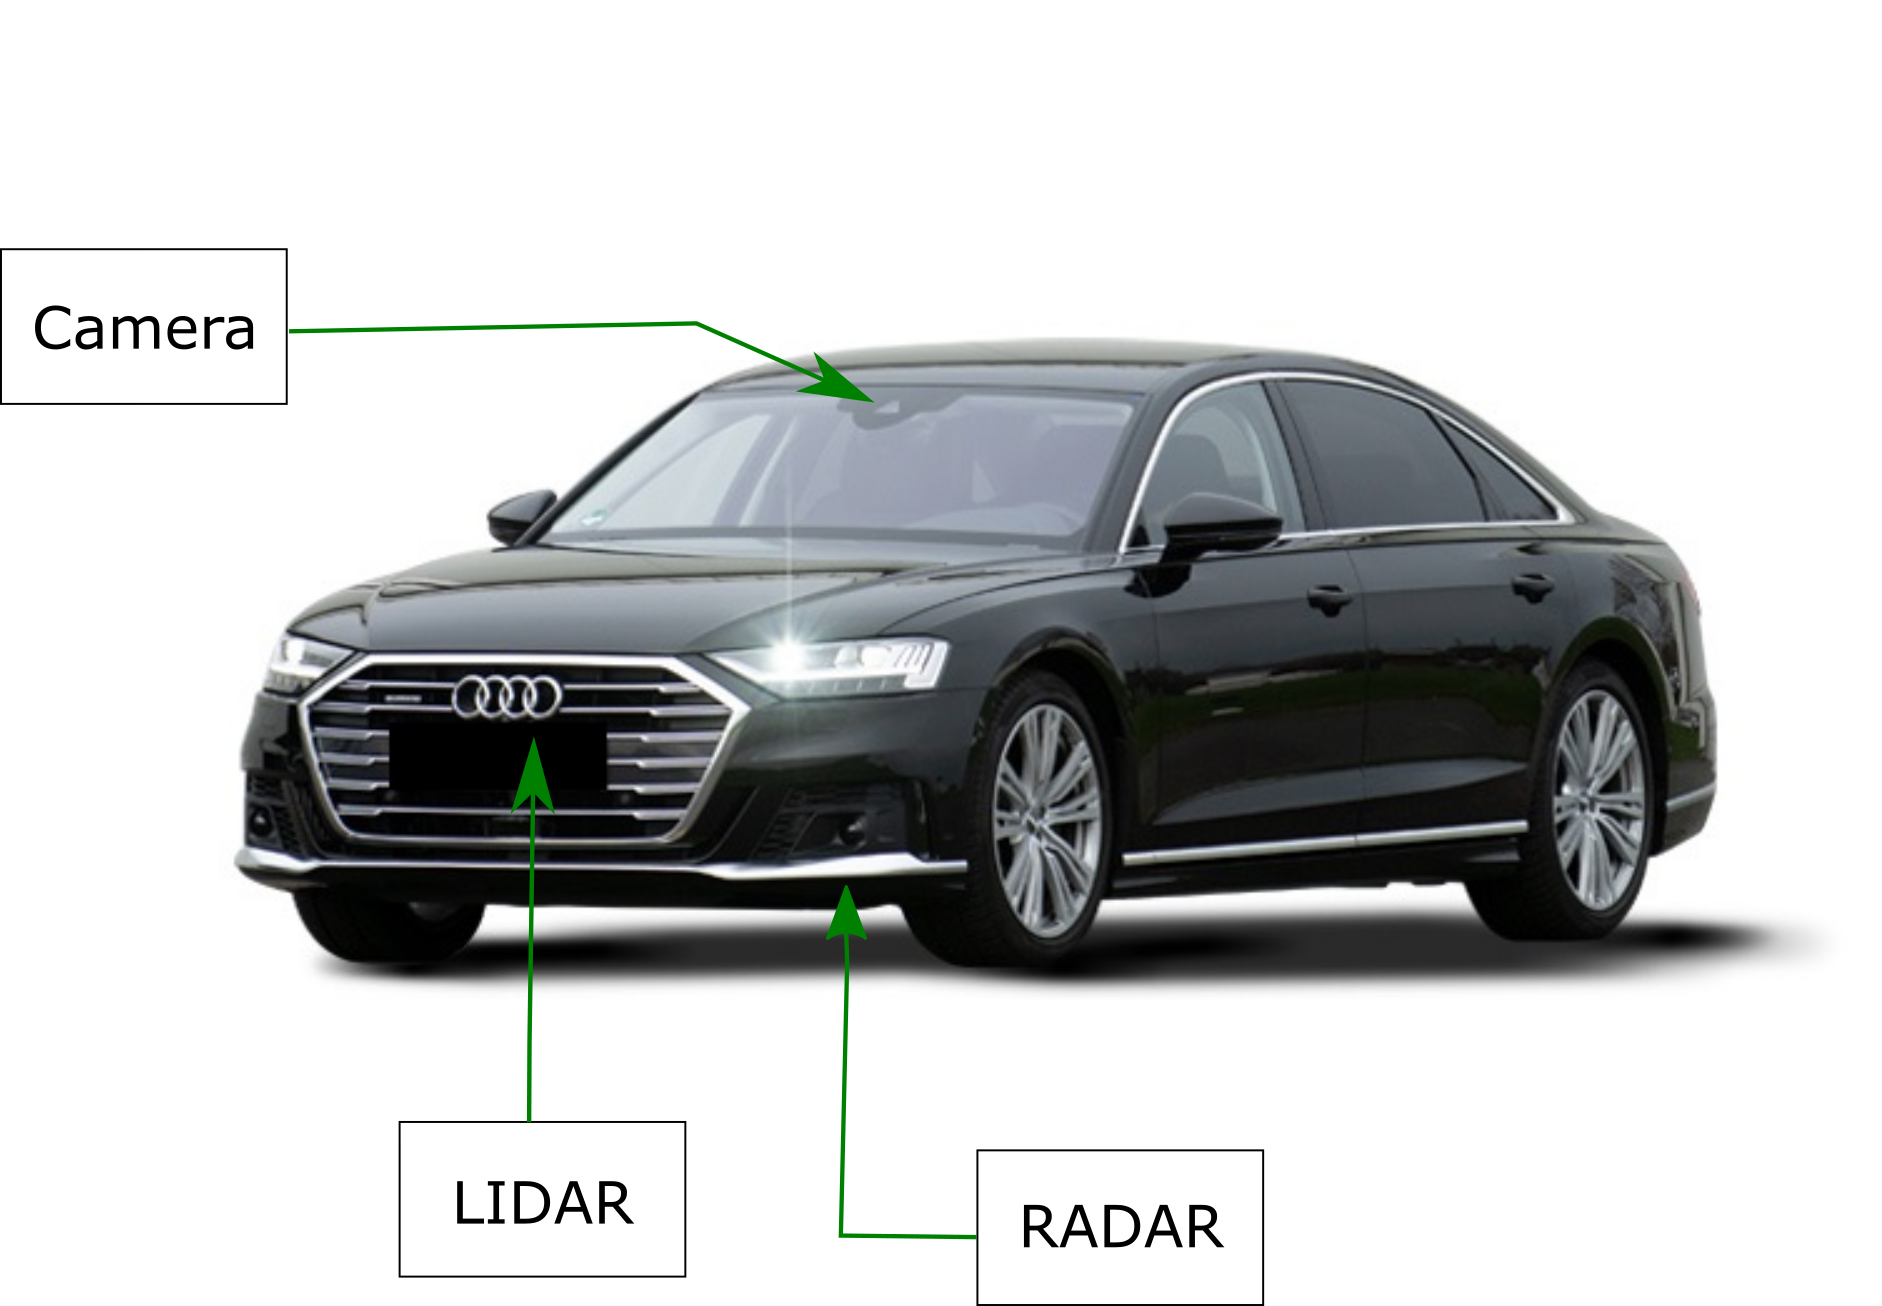
\includegraphics[scale=0.6]{imagens/image823.png}
\caption{Representation of an autonomous vehicle}
\label{fig:autonomous-vehicles}
\end{figure}


Each sensor has a different range and coverage angle, and this mixing of the sensor in the car allows it to cover a big area and make it possible to reduce car accidents and improve the driver's safety.  Although Figure \ref{fig:sensorsrange} shows reasonable performance parameters for AV sensors, specific sensor designs and implementations will ultimately determine the performance parameters for a particular AV in the real world.


\begin{figure}[H]
\centering
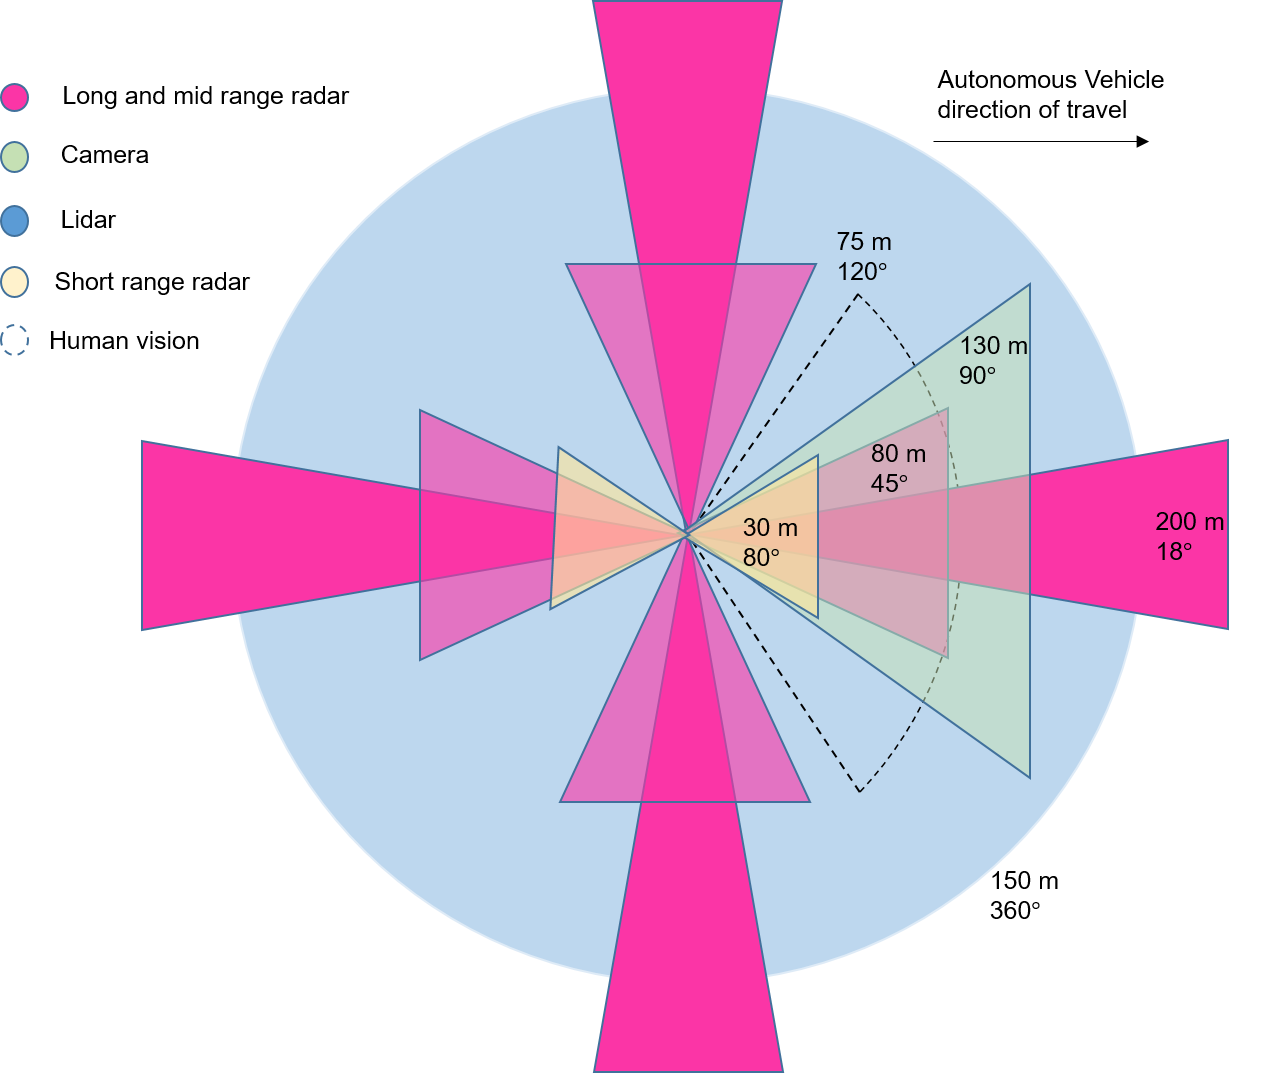
\includegraphics[scale=0.7]{imagens/Imagem1.png}
\caption{Illustration of the various sensors, with reasonable estimates of coverage area (field of view) and typical operating ranges}
\label{fig:sensorsrange}
\end{figure}



\subsubsection{Camera}\label{sub:camera}
The camera is the type of sensor that allows the car to perceive the environment using the collected images. Figure \ref{fig:camera} shows the standard camera for autonomous vehicles.

It is an optical instrument for image or video capture in the same size. For example, there are some cameras where it is possible to set up the numbers of frames per second (FPS) and the image resolution. 

It is also essential to remember the importance of the camera's calibration; the Equations for this process were available in \cite{888718}. This step is necessary to acquire the objects' real size because it is sometimes required to compare these objects' dimensions. 

\begin{figure}[H]
\centering
\includegraphics[width=80mm]{imagens/camera.png}
\caption{Representation of a camera of the autonomous vehicle \cite{site-camera}}
\label{fig:camera}
\end{figure}

There are many different models of cameras, which vary in their technical specs. In this thesis, it uses GoPro5, which is the highest-end model. The camera alone weighs 118 g, and 186 g with the camera, we selected this camera because it works better for outside scenarios. GoPro gives the user great control of the settings for both picture and video acquisition. Video offers some recording options, from 480p until 4k resolution, at various frame rates. There is also the option to shoot in 4K—a resolution higher than most HD televisions. The user can also adjust exposure, white balance, color, ISO, and sharpness, among other settings \cite{paro2015video}.

GoPro carries a WiFi signal within itself that allows connected devices like another GoPro or your computer. There is no internal storage, and video is saved into removable microSD cards. Battery life is dependent on which video quality. The official Web site suggests a battery life of 2 hours of continuous video and three hours for recharging.

This sensor allows the car to detect many objects while it is possible to perform object recognition. It is necessary to freeze the difference between object detection and object recognition. There are different algorithms to perform these tasks. The proposed algorithm in Chapter \ref{capitulo4} shows both exposures combined with the estimation of the distance. 

\subsubsection{Radar}\label{sub:radar}

The automotive radio detection and ranging (RADAR) sensors are responsible for performing object detection around the vehicle and avoiding potential collisions. Therefore, with this sensor, it is possible to warn the driver and combined with level 1 of automation, as shown in Figure \ref{fig:automation}, to intervene with the brake the car or use other controls to prevent an accident \cite{ariyur2006collision}.

\begin{figure}[H]
\centering
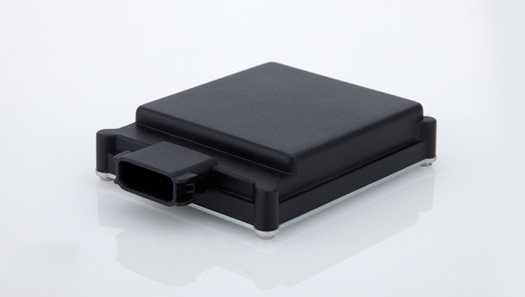
\includegraphics[width=120mm]{imagens/radar.jpg}
\caption{A commercial radar model ARS430 CV from Continental}
\label{fig:camera}
\end{figure}

Another exciting application of the RADAR in the automotive scenario is measuring the vehicle's relative speed and other objects. It is possible to estimate the distance correctly  \cite{stevenson2011long}.

It is possible to combine the camera and RADAR and get a new kind of sensor, as defined in \cite{kamerad}. With this approach, it is possible to reach 160 times faster than a human driver.

\subsubsection{Lidar}\label{sub:lidar}
In Figure \ref{fig:lidar} is shown a light detection and ranging (LIDAR). The main purpose of this laser is to detect and track any kind of objects. 
\begin{figure}[H]
\centering
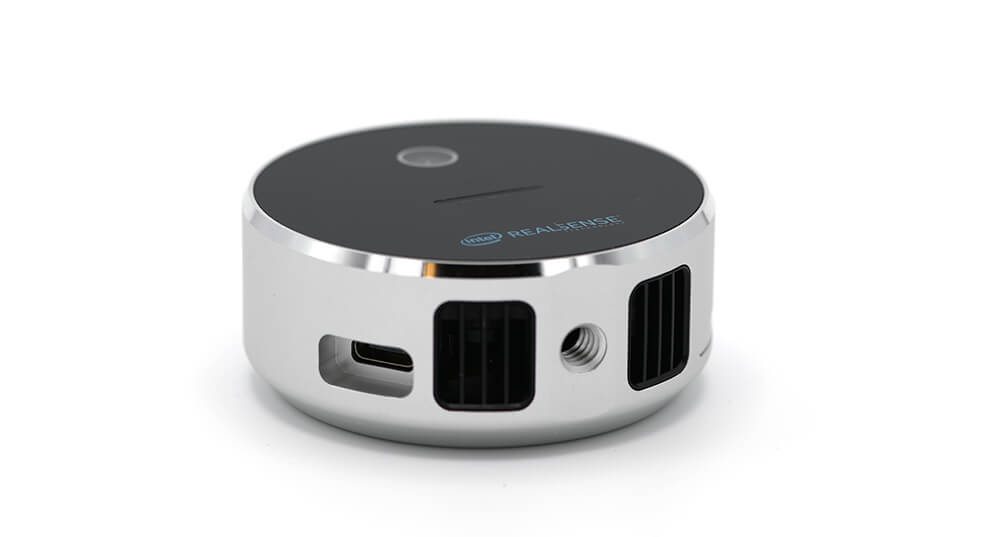
\includegraphics[width=\columnwidth]{imagens/lidar.jpg}
\caption{An exemple of a lidar of the autonomous vehicle}
\label{fig:lidar}
\end{figure}

This measurement is based on many times rotate this sensor in different directions to scan the whole area of the autonomous vehicles is driving and collect some data for detecting the objects \cite{gao2018object}.

\section{Machine Learning in Computer Vision}\label{ml-ai}
The machine learning is an approach based on algorithms to create some predictions. These techniques are based on mathematical and computer science. It is possible to apply this in several fields of science. 
\subsection{Artificial Neural Networks}

The human brain has inspired artificial neural networks (ANN) or perceptron. This approach is because of the capacity of the human mind to categorize new information. In Figure \ref{fig:ann} is shown an example of the structure of an ANN. There is an input array with the processed features for categorization. The next step of the processing is to define the weights for this analysis. The activation function is the central part of this process. In this step, the algorithm will transform the numbers collected by the previous actions and return only in twofold purpose, like $0$ and $1$ in the output layer \cite{goodfellow2016deep}.

\begin{figure}[H]
\centering
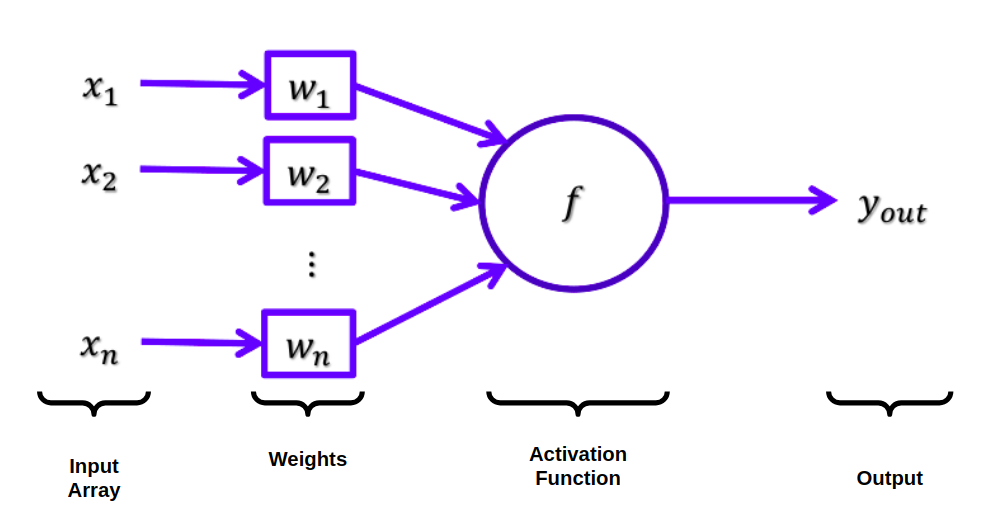
\includegraphics[width=\columnwidth]{imagens/ann.png}
\caption{The structure of an ANN \cite{lecture}}
\label{fig:ann}
\end{figure}

The neuron output is a function of the weighted sum of its inputs. Figure \ref{fig:ann_weight} is shown the mathematical background, where $f$ is activation function, $w_i$ are the weights, and $\beta$ is the constant input called bias.


\begin{figure}[H]
\centering
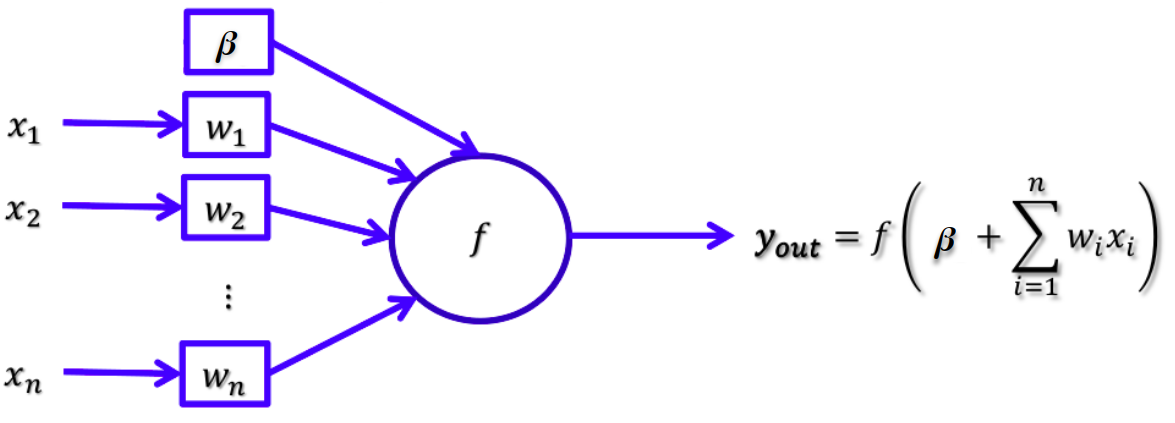
\includegraphics[width=\columnwidth]{imagens/math_ann_bias.png}
\caption{Mathematical representation of ANN with bias \cite{lecture}}
\label{fig:ann_weight}
\end{figure}


\subsubsection{Activation functions}
There are many different activation functions to use. These are crucial for ANN characteristics, such as learning ability and computational efforts in training and validation.

There are different kinds of activation functions for machine learning approaches. Each activation function has its particularity for specific problems. Table \ref{tab:tab1} shows the characteristics for these functions. 


\begin{table}[H]
\caption{Comparison Table for Activation Functions}
\centering
\resizebox{15.3cm}{!}{%
\begin{tabular}{|c|c|c|c|c|c|c|}
\hline
\textbf{\begin{tabular}[c]{@{}c@{}}Activation\\ Function\end{tabular}}  & \textbf{Linear}          & \textbf{Monotonic} & \textbf{Continuous}      & \textbf{\begin{tabular}[c]{@{}c@{}}Derivative \\ Monotonic\end{tabular}} & \textbf{\begin{tabular}[c]{@{}c@{}}Derivative\\ Continuous\end{tabular}} & \textbf{\begin{tabular}[c]{@{}c@{}}Simetric with \\ respect to \\ The Origin\end{tabular}} \\ \hline
{\color[HTML]{000000} Unit Step} & {\color[HTML]{FE0000} x} & {\color[HTML]{009901} \checkmark}& {\color[HTML]{FE0000} x} & {\color[HTML]{FE0000} x} & {\color[HTML]{FE0000} x} & {\color[HTML]{FE0000} x} \\ \hline
Sign & {\color[HTML]{FE0000} x} & {\color[HTML]{009901} \checkmark}& {\color[HTML]{FE0000} x} & {\color[HTML]{FE0000} x} & {\color[HTML]{FE0000} x} & {\color[HTML]{009901} \checkmark} \\ \hline
Identity & {\color[HTML]{009901} \checkmark}& {\color[HTML]{009901} \checkmark}& {\color[HTML]{009901} \checkmark}& {\color[HTML]{FE0000} x} & {\color[HTML]{009901} \checkmark}& {\color[HTML]{009901} \checkmark}\\ \hline
Sigmoid                                                                 & {\color[HTML]{FE0000} x} & {\color[HTML]{009901} \checkmark}             & {\color[HTML]{009901} \checkmark}                   & {\color[HTML]{FE0000} x}                                                 & {\color[HTML]{009901} \checkmark}                                                                   & {\color[HTML]{FE0000} x}                                                               \\ \hline
\begin{tabular}[c]{@{}c@{}}Hyperbolic\\ Tangent\end{tabular}            & {\color[HTML]{FE0000} x} & {\color[HTML]{009901} \checkmark}             & {\color[HTML]{009901} \checkmark}                   & {\color[HTML]{FE0000} x}                                                 & {\color[HTML]{009901} \checkmark}                                                                   & {\color[HTML]{009901} \checkmark}                                                                                 \\ \hline
\begin{tabular}[c]{@{}c@{}}Rectified \\ Linear Unit \\ (ReLU)\end{tabular} & {\color[HTML]{FE0000} x} & {\color[HTML]{009901} \checkmark}              & {\color[HTML]{009901} \checkmark}                   & {\color[HTML]{009901} \checkmark}                                                                   & \begin{tabular}[c]{@{}c@{}}{\color[HTML]{FE0000} x}\\ (at 0)\end{tabular}                       & {\color[HTML]{FE0000} x}                                                               \\ \hline
\end{tabular}\label{tab:tab1}}
\end{table}


Equation \ref{eq:eq_unit} shows the behavior of the Unit Step activation function ($H(x)$) where it is possible to note that it is nonlinear, monotonic, and adequate for classification. However, on the other hand, it has discontinuous derivatives and not monotonic with gradient descent methods.


\begin{equation}\label{eq:eq_unit}
    H(x) = \left\{\begin{matrix}
    1 & if & x >  0,\\
    \frac{1}{2} & if & x = 0, \\
    0 & if & x < 0 
    \end{matrix}\right.
\end{equation}

Equation \ref{eq:sign} shows the behavior of the Sign Function activation function. Its properties are similar to the (\ref{eq:eq_unit}) as they have, essentially, the same format with different values. The pros are nonlinear, monotonic, and ideal for fine classification, but the cons are discontinuous and not suitable for regressions.


\begin{equation}\label{eq:sign}
    sgn(x) = \left\{\begin{matrix}
    1 & for & x >  0,\\
    0 & for & x = 0, \\
    -1 & for & x < 0 
    \end{matrix}\right.
\end{equation}

        


Equation (\ref{eq:identity}) defines the Identity activation function where the usage is indicated when necessary to optimize the weights, but for multilayers networks are not recommended because it is a linear function. 


\begin{equation}\label{eq:identity}
    f(x) = x
\end{equation}


Equation (\ref{eq:sigmoid}) shows the classic activation function for the multi-layer networks. It is important to remind that this function is nonlinear, monotonic, and well-suited to gradient descent, but its asymmetry to the origin may have slower convergence and can get stuck at the training time.     


\begin{equation}\label{eq:sigmoid}
    \mathrm{S}(x) = \frac{1}{1+e^{-x}}
\end{equation}

        
Equation (\ref{eq:hiper}) proposes an alternative to (\ref{eq:sigmoid}) where has a non-linearity and it is symmetric to its origin, and it is well suited to gradient descent optimization, but at the same, it does not have a monotonic derivative and can have a slow convergence, but it is better sometimes than the Sigmoid activation function.


\begin{equation}\label{eq:hiper}
 \mathrm{tanh}(x) = \frac{e^{x}-e^{-x}}{e^{x}+e^{-x}}
\end{equation}


    


In this work, ReLU is the activation function chosen activation. Its mathematical definition is shown in (\ref{eq:relu}). This activation function is a novel, and it is widely used in deep networks because it is nonlinear and has a fast convergence. Contrarily of the previous equations, it is not differential continuously just at zero, and the issues to work with gradient descent is just around the origin. 


\begin{equation}
\label{eq:relu}
    f(x) = \mathrm{R}(x) = \mathrm{max}(0,x)
\end{equation}


The graphic visualization of the function Relu is shown in Figure \ref{fig:relu}, where this function returns $0$ if the number from the weighted sum is lower than $0$, or return $x$ if the previous value is over than $0$.


\begin{figure}[H]
\centering
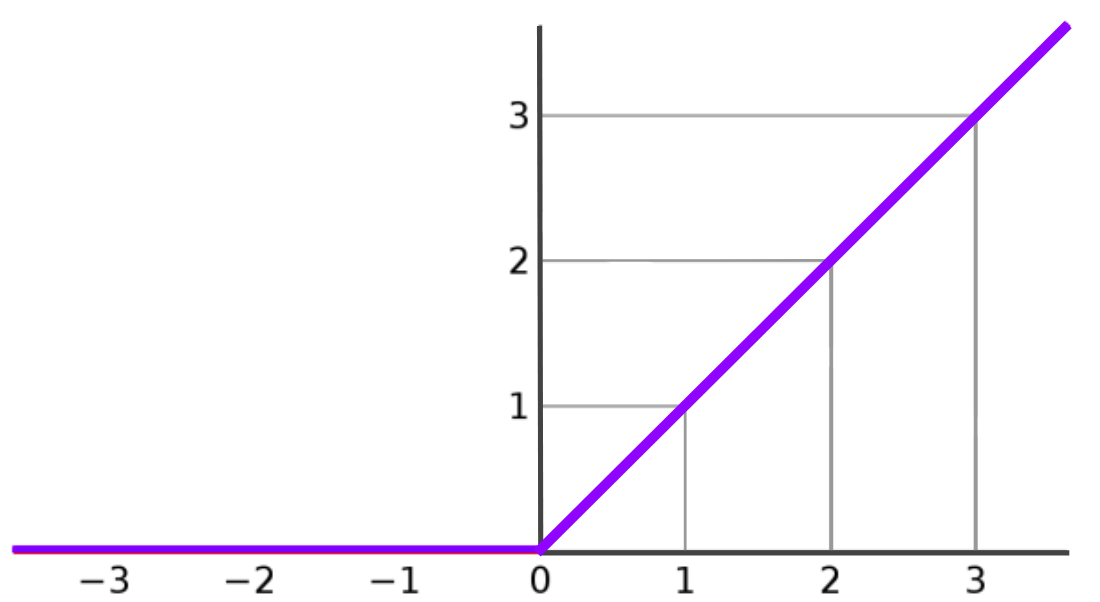
\includegraphics[scale=0.2]{imagens/relu_corrected.png}
\caption{The behavior of the Relu \cite{lecture}}
\label{fig:relu}
\end{figure} 

These are the essential characteristics of this activation function. It is widely used in deep networks. It is nonlinear, monotonic, derivative monotonic, and fast converge. As the weaknesses, this activation function has a non continuously differential at zero, i.e., issues with gradient descent around the origin.



\subsubsection{Layered Neural Networks}

The quintessential element of a deep learning model is the multilayer perceptron (MLP) ~\cite{goodfellow2016deep}. An MLP is just a mathematical function mapping some set of input values to output values. The function
is formed by composing many more specific functions \cite{goodfellow2016deep}.


These are important deep learning models. The goal
of a feedforward network is to approximate some function $f*$. For example, for a classifier, $y = f*(x)$ maps an input x to a category y. A feedforward network
defines a mapping $y = f (x; \theta)$ and learns the value of the parameters $\theta$ that result in the best function approximation.

These models are called feedforward because information flows through the function being evaluated from $x$, through the intermediate computations used to define $f$, and finally to the output $y$. There are no feedback connections in which results of the model are fed back into itself.



\subsection{Convolutional Neural Networks}\label{sec:cnn}


The Convolutional Neural Networks (CNN) is a specialized neural network for processing data known as in \cite{lecun1995convolutional}. For example, in the autonomous vehicle domain, this approach is several used for object detection and object identification. This name  indicates that the network employs a mathematical operation called
convolution. 

A CNN coarsely scans the image for features (in lower dimension space), pools possible patterns, then inspect those patterns in detail with its fully connected
subnetworks, generating their classifications. In Figure \ref{fig:cnn_car} is defined the full process of this neural network. Where there are three other importants is steps: Convolutional layer is defined in Subsection \ref{sub:conv}. The pooling layer is introduced in the Subsection \ref{sub:pooling}.
\begin{figure}[H]
\centering
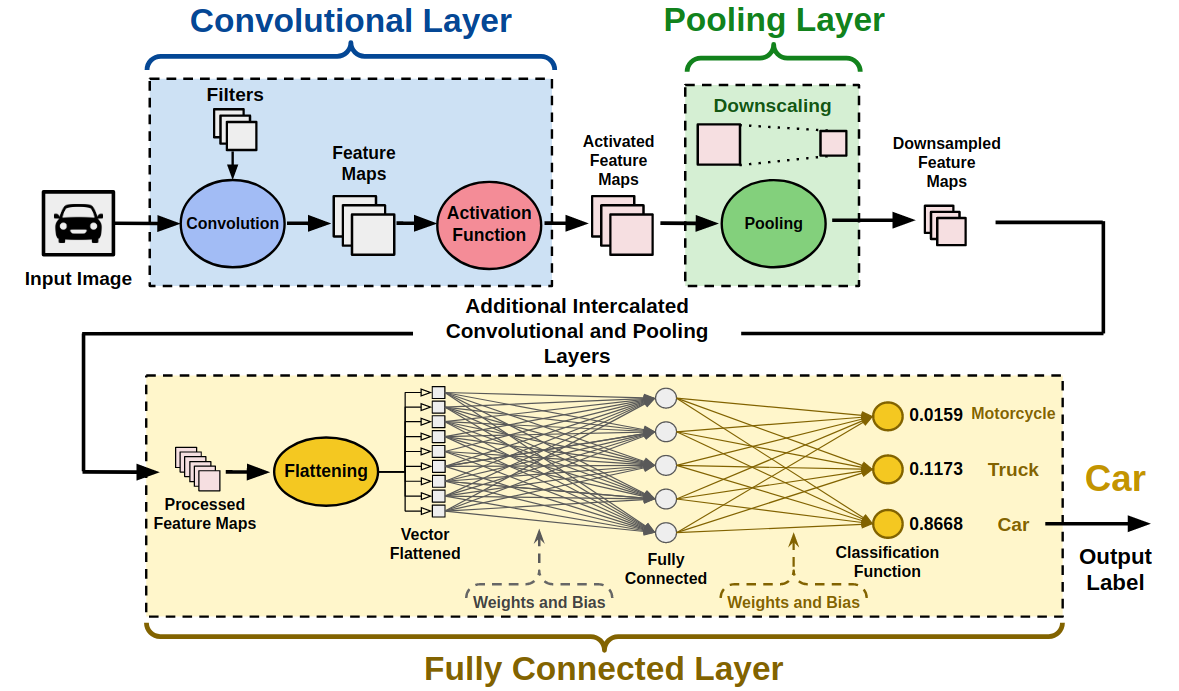
\includegraphics[width=\columnwidth]{imagens/Full_Process.png}
\caption{Full process of a convolutional neural network \cite{lecture}}
\label{fig:cnn_car}
\end{figure}


\subsubsection{Convolutional Layer}
\label{sub:conv}

The standard inputs are a tridimensional matrix with height and width defined accordingly with the image dimensions and determined by the number of colors. In general, the images use three color channels, Red-Green-Blue (RGB), as is shown in Figure \ref{fig:rgb}.

\begin{figure}[H]
\centering
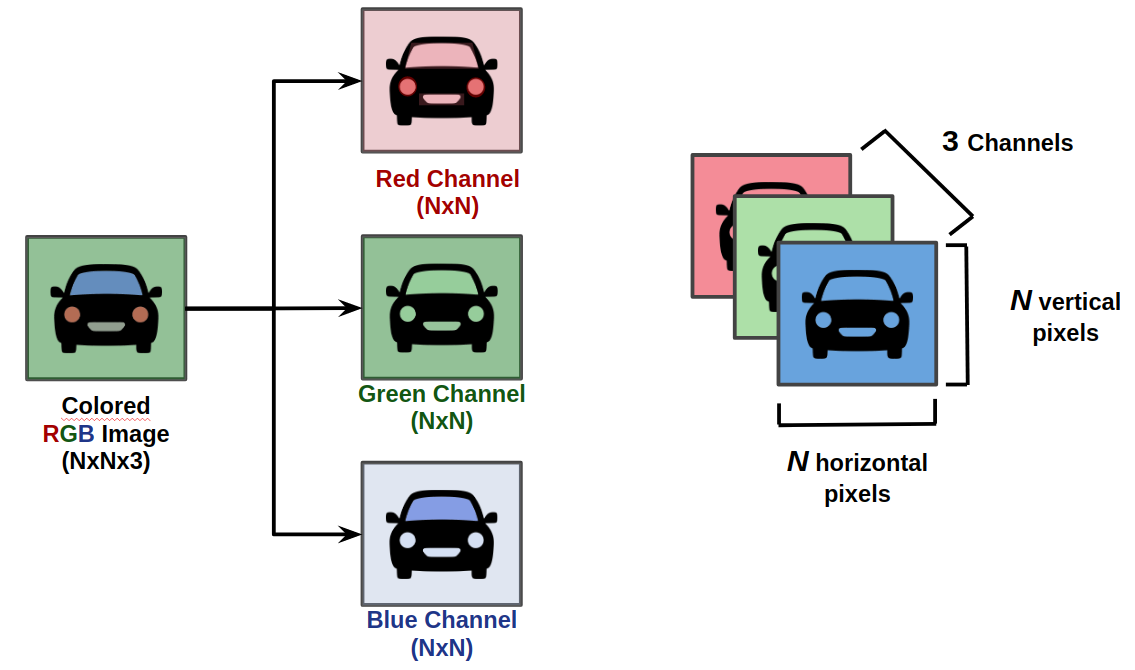
\includegraphics[scale=0.35]{imagens/rgb_representation.png}
\caption{Representation of the colors of the input image \cite{lecture}}
\label{fig:rgb}
\end{figure}


The convolutions work as filters that seem little squares, and they are slipping through the whole image and capturing essential parts.  Figure \ref{fig:bias} shows an image by dimensions of $NxNX3$, filter among the $MxMX3$, wherever individual main difference per result is then summed, on bias ($\beta$) value, then passed through an activation function. Furthermore, the end of the process generates a new matrix called a feature map or activation map.


\begin{figure}[H]
\centering
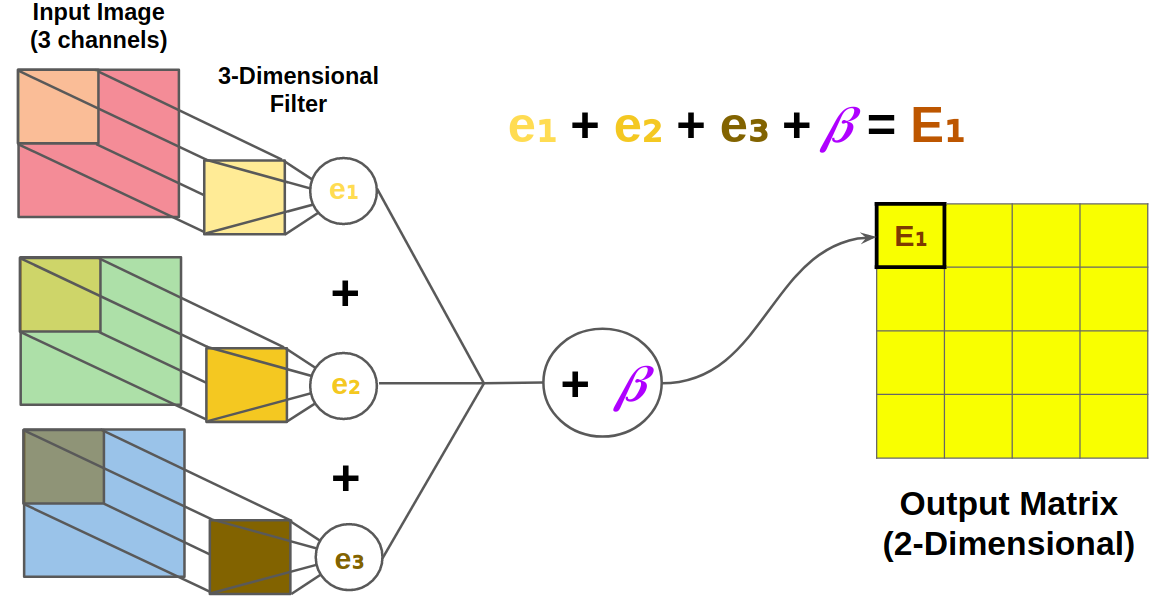
\includegraphics[scale=0.35]{imagens/three_dim_conv_2.png}
\caption{Representation of the convolution process \cite{lecture}}
\label{fig:bias}
\end{figure}




\subsubsection{Pooling and Upsampling}\label{sub:pooling}

A pooling layer is necessary to simplify the information from the previous layer. The convolution layer is choosing a unit area, for example, $2x2$, to slicing for the whole output information from the previous step. To brief, if the information from the previous layer was $4x4$, the output from the process of pooling will be $2x2$. Nevertheless, the most used method is max-pooling, where the biggest number in the matrix is passed to the next step. This data summarization is used to reduce the number of weights and avoid overfitting. In Figure \ref{fig:pooling} is shown the max-pooling process.

\begin{figure}[H]
\centering
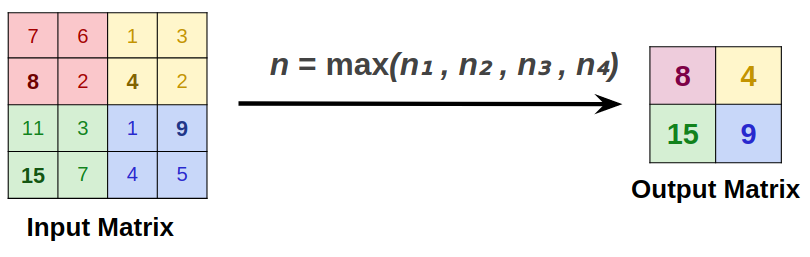
\includegraphics[scale=0.35]{imagens/max_pooling.png}
\caption{Representation of the maxpooling process \cite{lecture}}
\label{fig:pooling}
\end{figure}




\subsubsection{Auto-encoders}\label{auto-encoder}

It is a special type of neural network that is used to copy its inputs to its output. The intern structure is defined in Figure \ref{fig:autoencoder}. 

\begin{figure}[H]
\centering
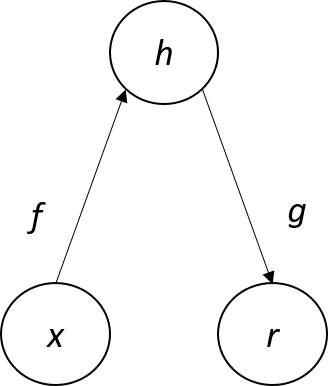
\includegraphics[scale=0.7]{imagens/autoencoder.png}
\caption{The structure of a standard autoenconder, where the variable $x$ means input and $r$ as an output through the internal representation in $h$. The encoder $f$ maps $x$ to $h$ and decoder $g$ maps $h$ to $r$}
\label{fig:autoencoder}
\end{figure}

As described in \cite{yang2020feedback}, this architecture has a hidden layer of $h$ that describes a code used to represent the input. The network may be viewed as consisting of two parts: an encoder function $h=f(x)$ and a decoder that produces a reconstruction $r=g(h)$.

\subsubsection{Training}

In the machine learning scenario, in special, the neural networks domain epoch can be defined as a single forward pass and backward pass of all the training examples. It feeds in all the neurons into the network at once. Instead, it chooses a batch of neurons and feeds them in. It performs stochastic gradient descent and prevents the system from overfitting. There is a difference between individual training step time and total training time \cite{pascanu2013difficulty}. 


